\section{Results}

At the conclusion of Run 3, in December of 2013, a total of 10 Bq of tritium was injected into LUX and removed. 300,000 events were observed in the 251 kg active volume of LUX, of which 170,000 events were in the 145 kg fiducial volume at the nominal LUX electric field of 180~V/cm. Another 4,500 fiducial events were collected in a special run at a reduced field of 105~V/cm. 

The LUX detector is described in detail in Ref. \cite{lux-nim}. Briefly, LUX is a cylindrical dual-phase TPC, with an array of 61 photomultiplier tubes (PMTs) immersed in the LXe at the bottom of the vessel, and an identical PMT array above the liquid-gas interface. Primary scintillation signals (S1) are detected on both arrays, while charge deposits drift vertically in the uniform drift field as established by anode and cathode wire grids. The charge deposits are extracted through the liquid-gas surface and create secondary scintillation (S2) before being collected by the anode. The spatial pattern of the S2 signals on the upper array localize the event in $x$ and $y$, while the drift time between S1 and S2 determines the $z$ coordinate.

Data is selected for analysis using cuts similar to the WIMP search analysis\cite{lux-reanalysis, lux-prd}. Within an event window, single scatters are selected by pairing an S1 with a single S2.  The S1 is measured with a spike-counting method that requires a minimum two-fold coincidence from PMTs that are not in neighboring channels. We correct the S1 and S2 signals for spatial and temporal variations such as the light collection efficiency and the free electron lifetime with $ ^{83m}$Kr data.  The S2 signal is required to be greater than 150 phd ($\sim$6 extracted electrons) to ensure accurate $x$-$y$ position reconstruction. Events are required to be within a fiducial volume between 38 and 305~$\rm \mu s$ in drift time (8.5 and 48.6 cm in the charge drift direction ($z$) measured from the face of the bottom PMTs) and less than 20~cm radius. In addition to the above selection cuts, which are applied to the WIMP search, in the tritium data we also reject events where the S2 signal is truncated by the end of an event buffer. This pathology is negligible in WIMP search data but is present at a small level in the tritium data due to the larger event rate.

\subsection{Tritium energy spectrum}

We interpret the data in terms of the combined energy model for electron recoils \cite{Platzman}, where the total energy of an event is directly proportional to the number of quanta produced (ionization electrons plus scintillation photons):

\begin{equation}
E_{total} = W \cdot (n_{\gamma} + n_e ),
\label{platzman_eq}
\end{equation}

\noindent
where $E_{total}$ is the energy of the deposition in keV and  $n_\gamma$ and $n_e$ are the number of photons and electrons respectively. We employ the combined energy model because it reproduces well the true energy of the event, while the individual photon and electron signals are non-linear in energy due to the effects of recombination. We use a $W$-value of 13.7 $\pm$ 0.2 eV/quanta \cite{Dahl_Thesis}. In LUX $n_{\gamma}$ and $n_e$ are proportional to the S1 and S2 signals, with gain factors $g_1$ and $g_2$: 

\begin{equation}
E_{total} = W \cdot \left(\frac{S1}{g_1} + \frac{S2}{g_2} \right),
\label{energy_eq}
\end{equation}

\noindent
where S1 and S2 have units of photons detected (phd) and $g_1$ and $g_2$ have units of phd per quantum. $g_1$ is the average light collection efficiency times the average quantum efficiency of the PMT arrays, while $g_2$ is the product of the electron extraction efficiency at the liquid-gas surface and the average single electron size in phd. For the December 2013 tritium dataset presented here, $g_1$ and $g_2$ are measured to be $0.115 \pm 0.005$ phd/photon and $12.1 \pm 0.9$ phd/electron. The constraint was set by allowing g1 and g2 to float and fitting the data to a true tritium spectrum \cite{Drexlin:2013lha}.  In the LUX Run 3 WIMP search, $g_1$ and $g_2$ are measured with line source data and single electron events to be $0.117 \pm 0.003$ phd/photon and $12.1 \pm 0.8$ phd/electron\cite{lux-reanalysis, lux-prd}, consistent with the values adopted here. 

\begin{figure}[h!]
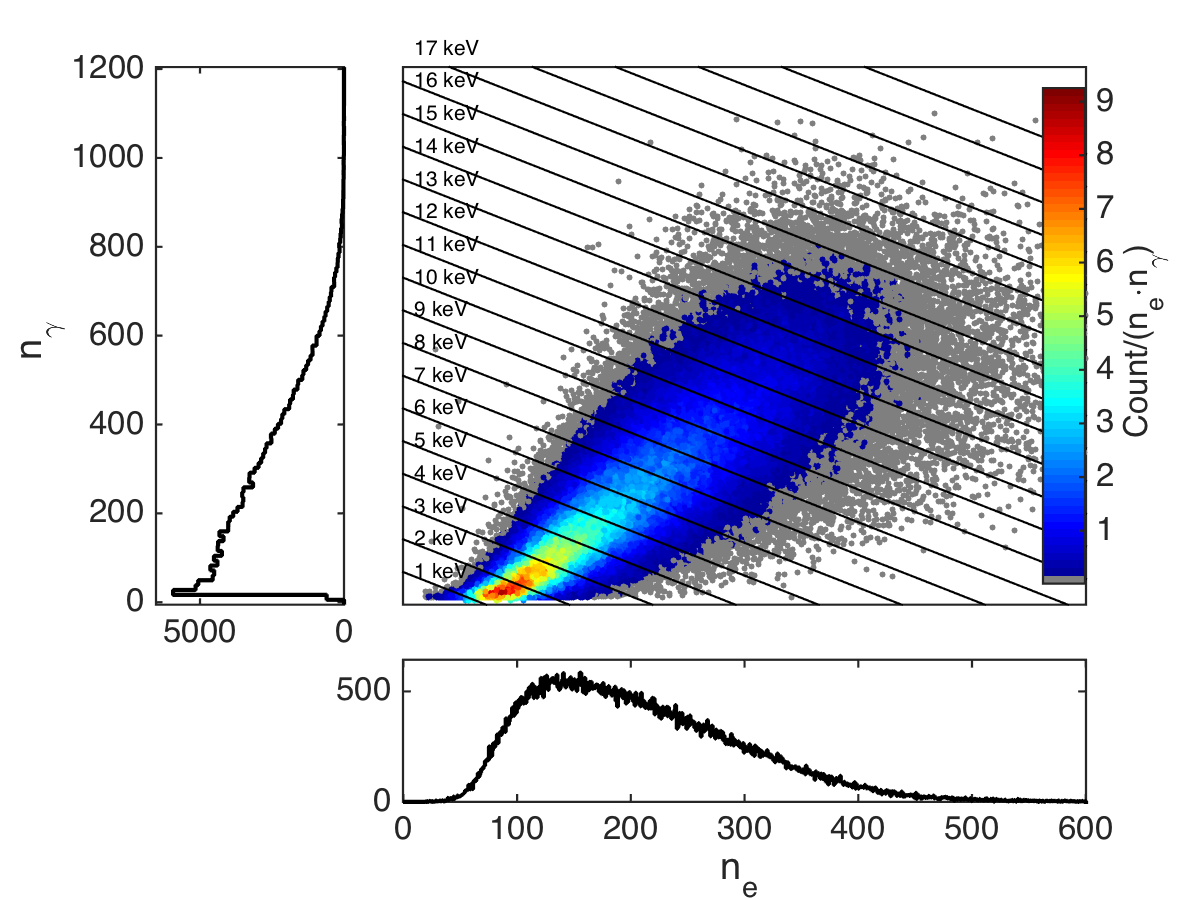
\includegraphics[width=90mm]{fig/tritium_scatter.png}
\caption{Scatter plot of $n_e$ vs $n_{\gamma}$ for 170,000 fiducial tritium events at 180~V/cm. Lines of constant energy are indicated assuming a $W$-value of 13.7~eV. The data is projected into $n_e$ and $n_{\gamma}$ histograms on each axis.}
\label{fig:tritium-scatter}
\end{figure}


\begin{figure}[h!]
\begin{center}
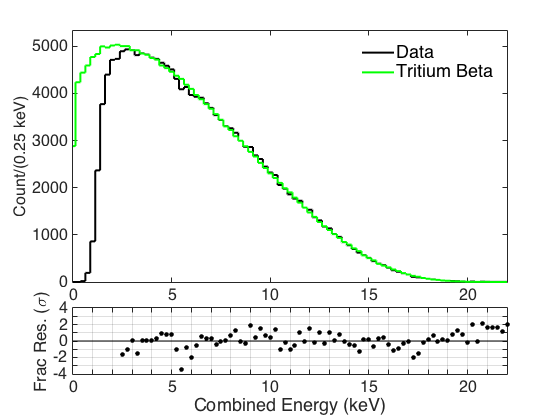
\includegraphics[width=90mm]{fig/tritium-spectrum-linear.png}
\caption{Top: The tritium energy spectrum measured by LUX with the combined energy model (black) compared to  a tritium spectrum convolved with detector resolution  ($\frac{\sigma_E}{W} = \sqrt{\sigma^2(n_{\gamma})+ \sigma^2(n_e)}$.) The p-value between data and model from 3 to 18 keV is 0.70. Bottom: Bin-by-bin fit residuals between data and theory, in units of $\sigma$. }
\label{fig:tritium-spectrum}
\end{center}
\end{figure}


A scatter plot of $n_e$ vs $n_{\gamma}$ for the tritium data at 180~V/cm is shown in Fig. \ref{fig:tritium-scatter}, along with the projected histograms on each axis. Contours of constant energy in 1~keV intervals are also plotted, derived from Eq. \ref{platzman_eq}. 

The tritium energy spectrum, obtained by projecting the data along the lines of constant energy, is shown in Fig. \ref{fig:tritium-spectrum}. The data are compared to a tritium spectrum with an energy smearing factor of $ \frac{\sigma_E}{W} = \sqrt{\sigma(n_{\gamma})^2 + \sigma(n_e)^2}$, where $ \sigma(n_{\gamma})$ and $ \sigma(n_e)$ represent the detector resolution for photon and electron counting. In the fit the models are normalized to the data. The ratio of the data to the smeared theoretical spectrum is shown in Fig. \ref{fig:ER-threshold}, along with an empirical fit to an error function. The effective 50\% energy threshold for ER events is found to be 1.24 $\pm$ 0.026~keV. The excellent agreement between data and theory from 3~keV to the endpoint of the tritium spectrum provides powerful support for the combined energy model of Eq.~\ref{platzman_eq}.

\begin{figure}[h!]
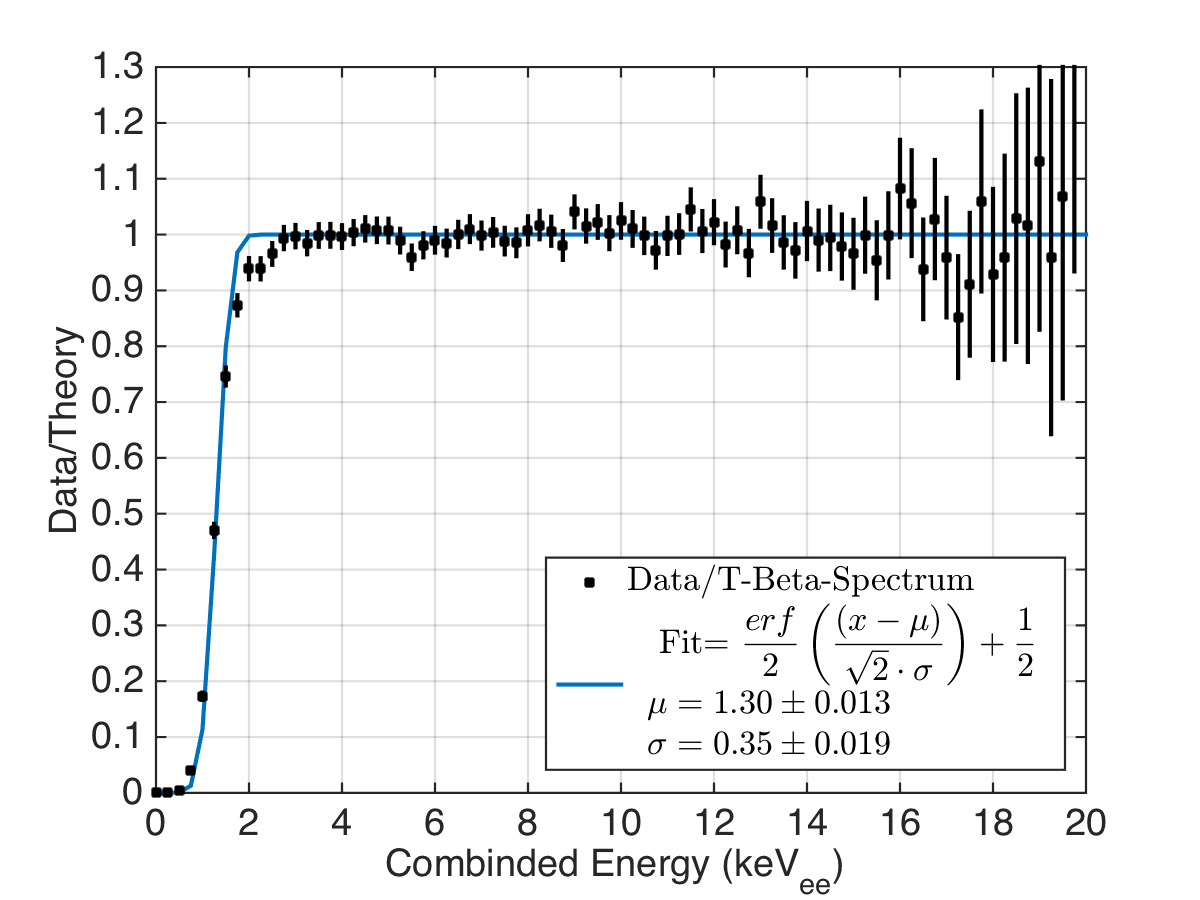
\includegraphics[width=90mm]{fig/E_Thres_Fit.png}
\caption{Ratio of the measured tritium energy spectrum and the true one convolved with the detector resolution. A fit to an error function is shown.}
\label{fig:ER-threshold}
\end{figure}

\subsection{Light and charge yields}

The mean light and charge yields of ER events in LUX are obtained by dividing the mean light and charge signals by the combined energy in each energy bin. The result is shown for 180~V/cm and 105~V/cm in Fig. \ref{fig:ER-LY-QY} along with NEST v0.98 model predictions at each field \cite{NEST_2013}. For these plots a small correction has been applied to the data to account for smearing of tritium events across energy bins due to the energy resolution and the spectral shape \cite{Dobi_Thesis}\footnote{We have verified with an internal $\rm ^{83m}Kr$ calibration source that the light yield of LXe is unaffected by the presence of CH$_4$ at concentrations up to $\sim$1 part per million. For the CH$_3$T measurements reported here the concentration was ($<$ $10\times10^{-12}$ g/g). }.  NEST v0.98 describes the data approximately, but predicts too much light yield and too little charge yield above 6~keV. Note that NEST v0.98 lacks direct input measurements in this energy range and electric field, so a modest disagreement is not unexpected. A more recent version of NEST (v1.0) has been tuned to reproduce the LUX tritium data shown here faithfully. The yield measurements at 180~V/cm and 105~V/cm are also listed in Tables \ref{table:Yields} and \ref{table:Yields_100} in Appendix \ref{sec:appendix3}.

\begin{figure}[h!]
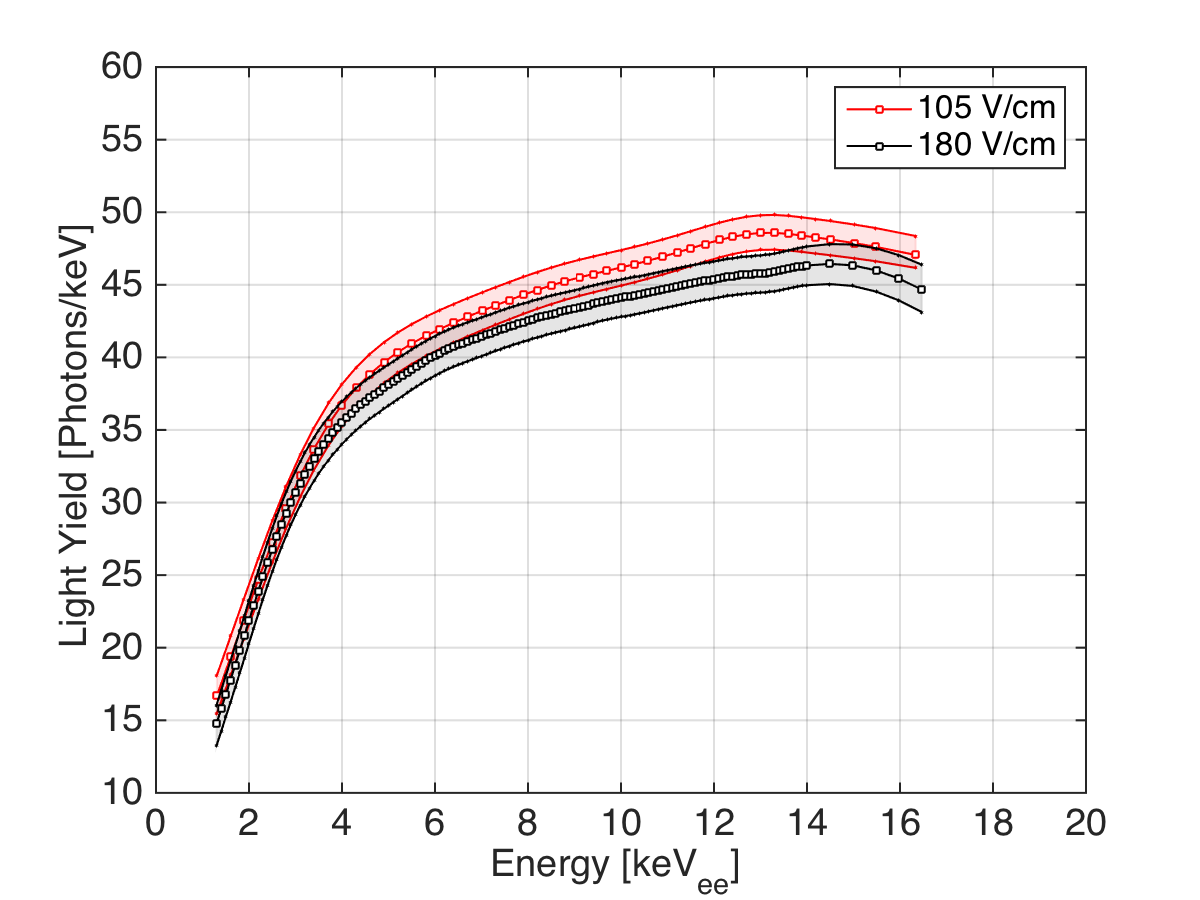
\includegraphics[width=90mm]{fig/ER_LY.png}
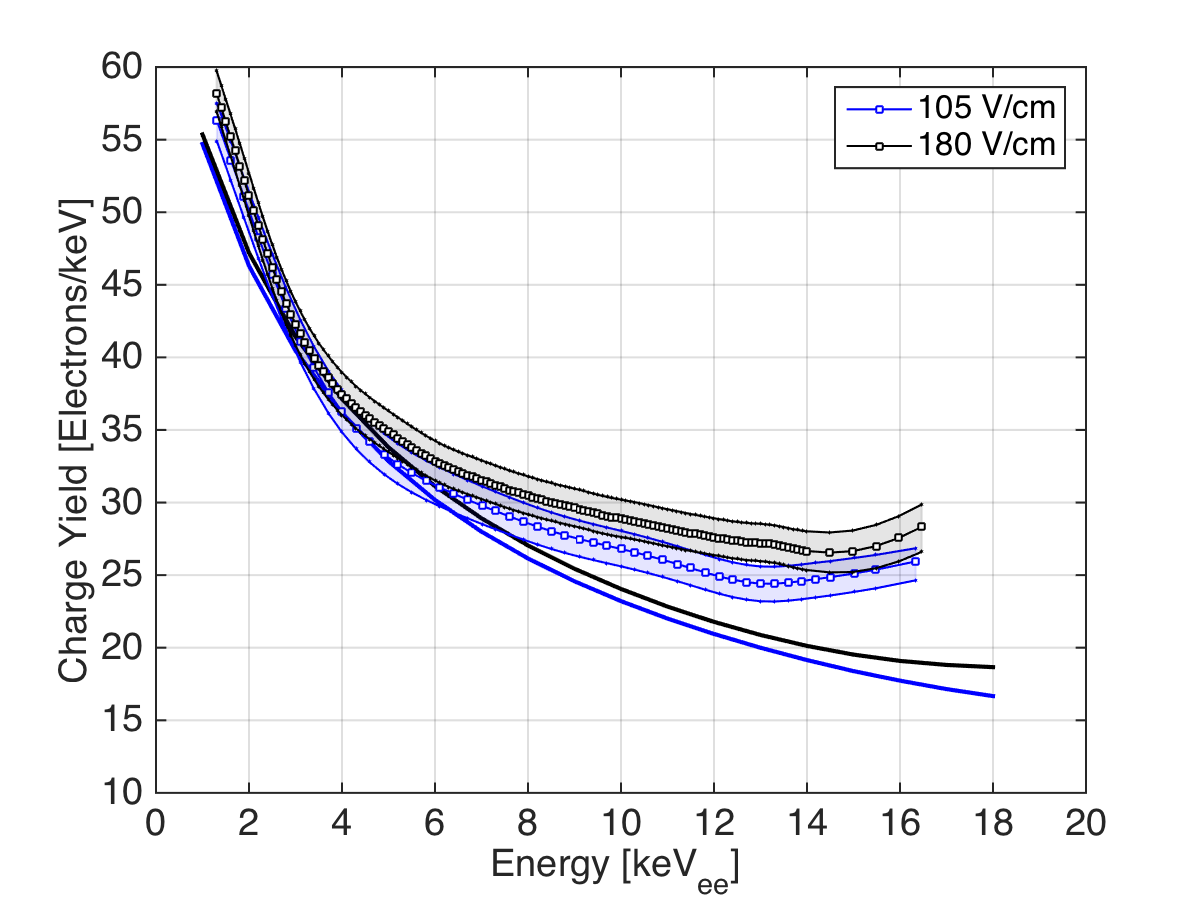
\includegraphics[width=90mm]{fig/ER_QY.png}
\caption{The light yield (upper plot) and charge yield (lower plot) of tritium ER events in LUX at 180~V/cm (black) and 105~V/cm (blue) compared to NEST v0.98 (2013) \cite{NEST_2013}. The NEST curves are solid red and dashed magenta for 180 and 105 V/cm respectively, with triangle markers spaced every one keV. The bands indicate the systematic errors due to $g_1$ and $g_2$, which are fully anti-correlated between the charge yield and light yield across all energy bins. }
\label{fig:ER-LY-QY}
\end{figure}

The light yield measurements are compared to similar measurements by other authors in Fig. \ref{fig:Re_LY}. To remove detector effects from this comparison, the light yield is normalized to that of the 32.1~keV electron capture decay of $\rm ^{83m} Kr$ at zero electric field. For LUX this light yield is measured to be $ 63.3 \pm 3$ photons/keV. Although the error bars on the comparison data are large, the findings are consistent with the expectation that the tritium light yields at 105 and 180~V/cm lie between those at zero field and 450~V/cm from \cite{Aprile_LY} and \cite{Baudis}. It is worth noting that Refs. \cite{Aprile_LY} and \cite{Baudis} use Compton scatters as the source of ER events, while in tritium data the ER source is a beta decay. At low energy beta decays and Compton scatters will leave similar track lengths and produce similar event characteristics. The comparison of Fig. \ref{fig:Re_LY} supports this expectation, albeit with large experimental uncertainties.

\begin{figure}[h!]
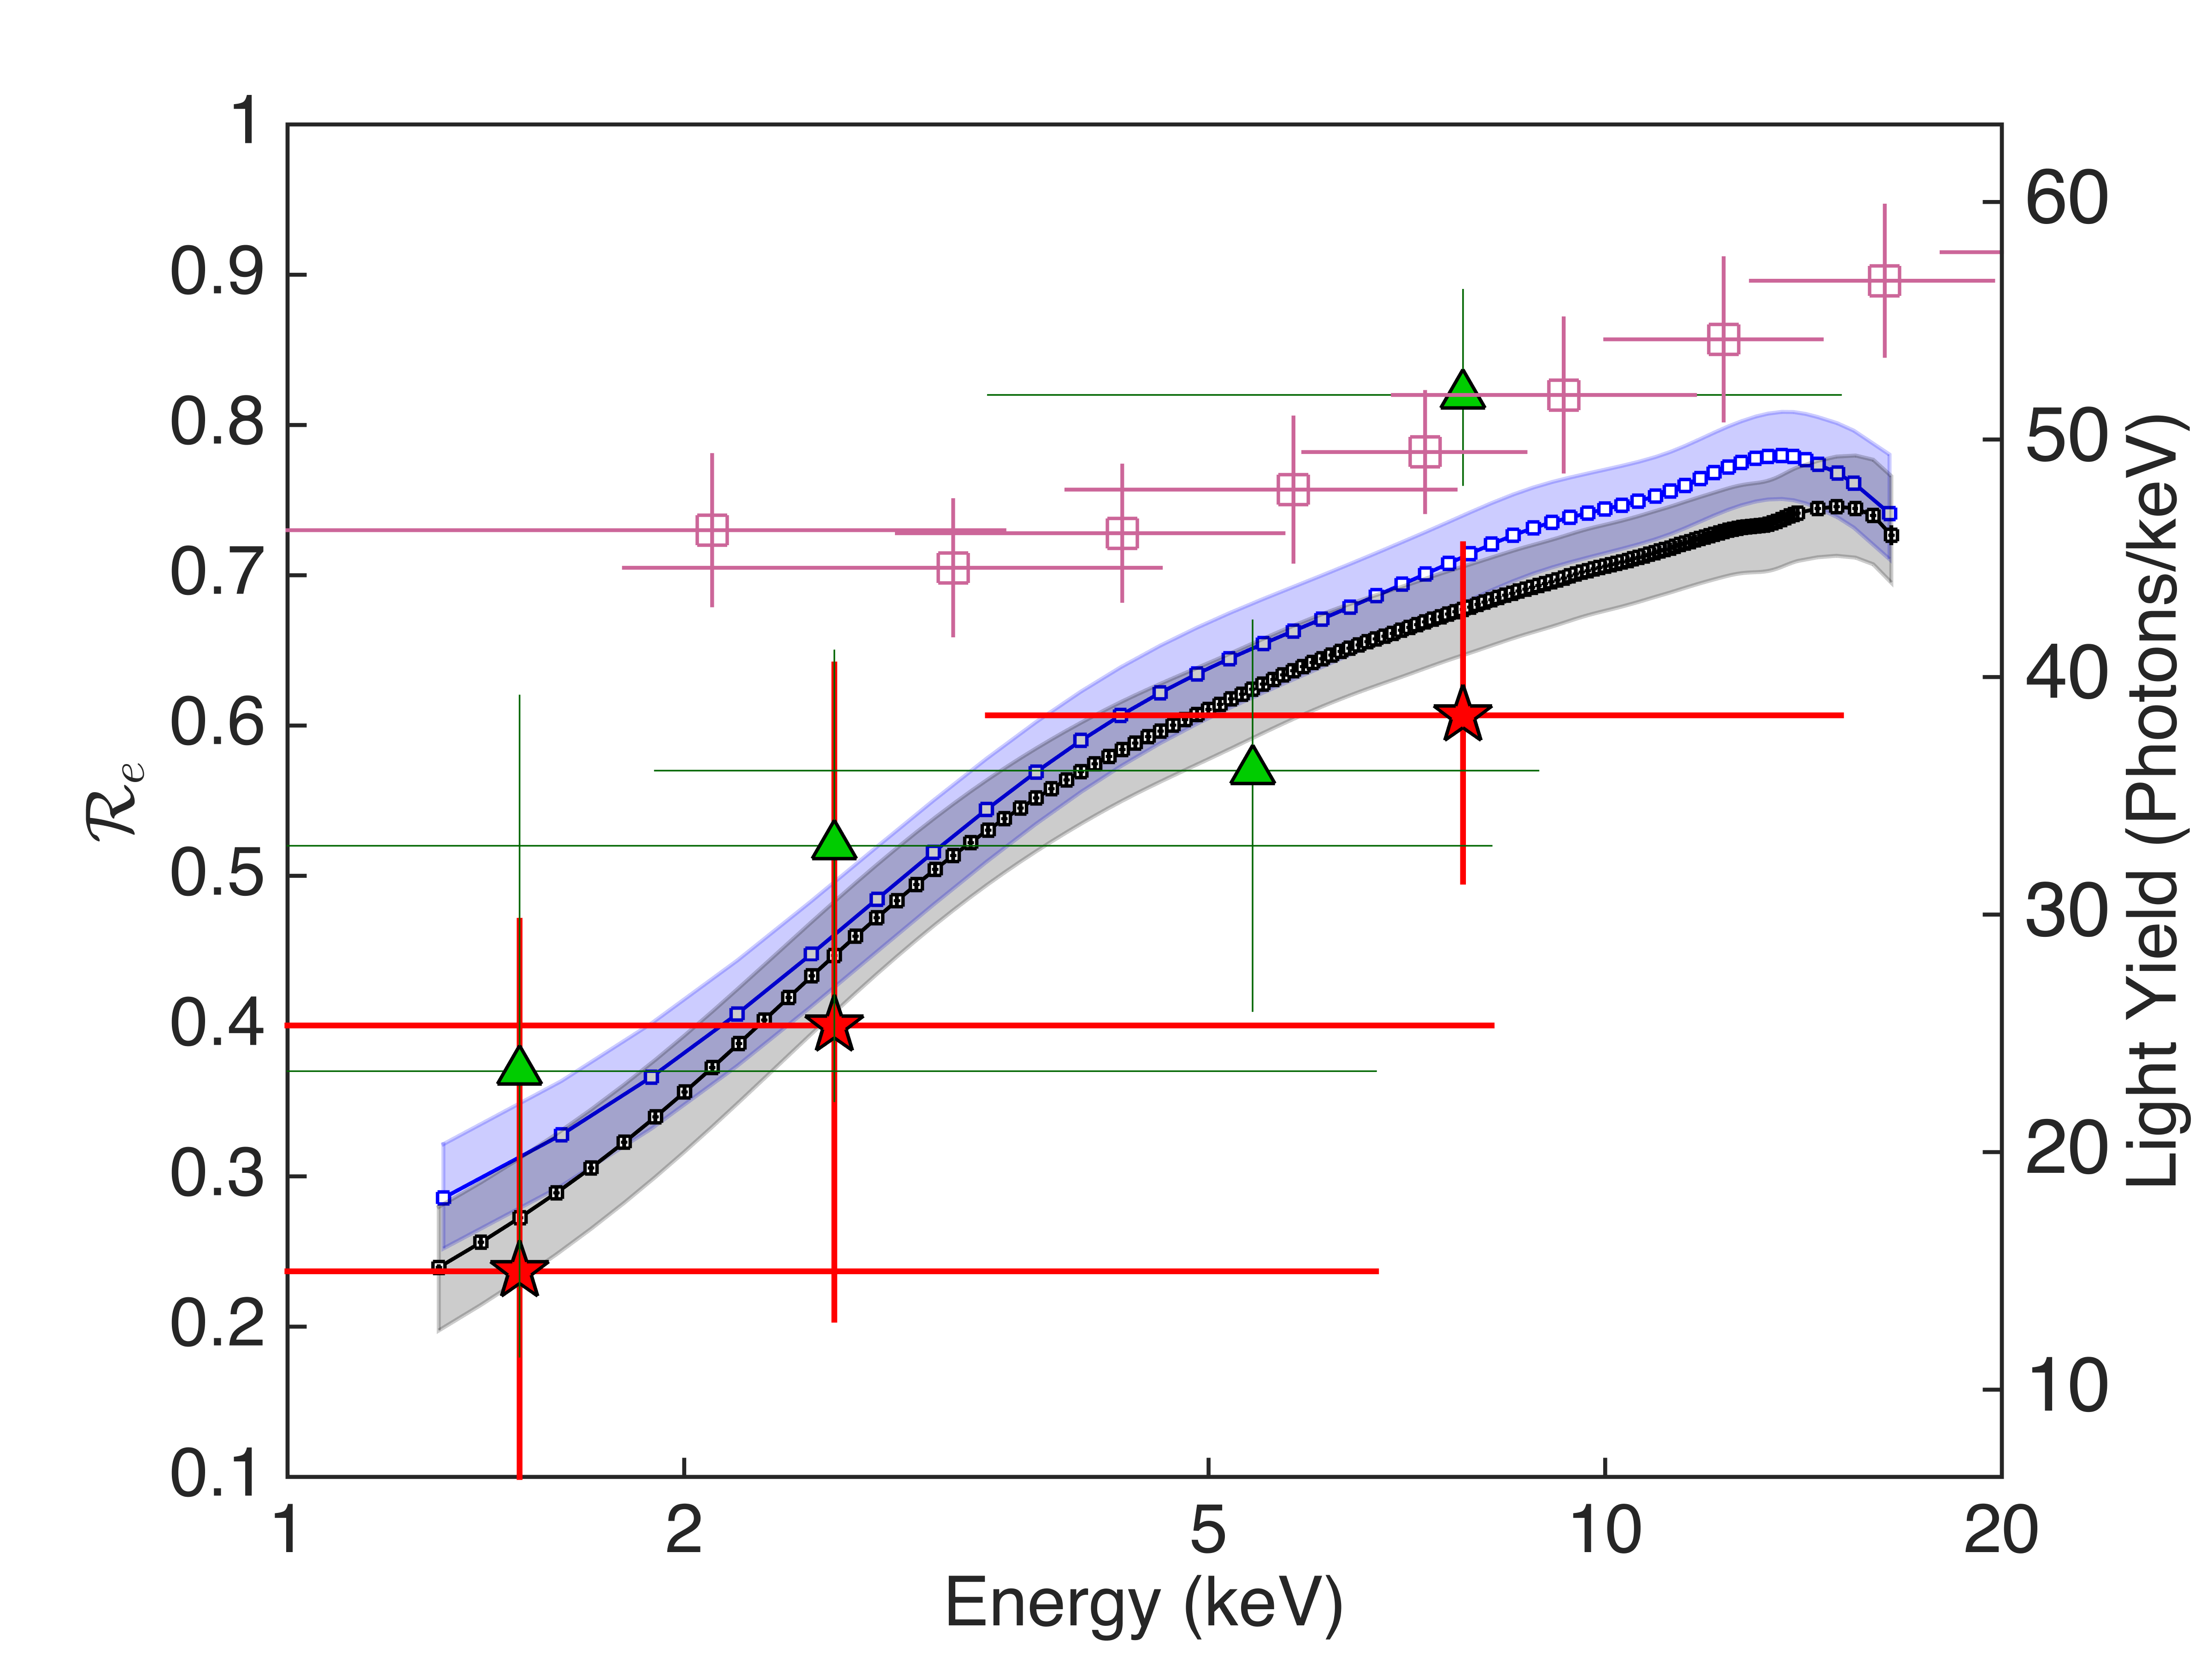
\includegraphics[width=88mm]{fig/Re_LY_log.png}
\caption{Light yield measurement from LUX tritium data compared with results from other authors. Left vertical scale: light yield relative to that of the 32.1~keV decay of $\rm ^{83m}Kr $ at zero field. Right vertical scale: absolute light yield measurements. Shaded blue curve is tritium at 105~V/cm, shaded black curve is tritium at 180~V/cm. Magenta squares represent zero field measurements from \cite{Aprile_LY}, cyan triangles and red circles represent zero field and 450~V/cm from \cite{Baudis}. All non-tritium data is from Compton scatters. }
\label{fig:Re_LY}
\end{figure}


As shown in Fig. \ref{fig:ER-LY-QY}, we find that the light yield increases rapidly from 1 to 6~keV, and then becomes less energy dependent over the remainder of the tritium spectrum. The charge yield exhibits the reverse behavior, in agreement with the combined energy model. 

\begin{figure}[h!]
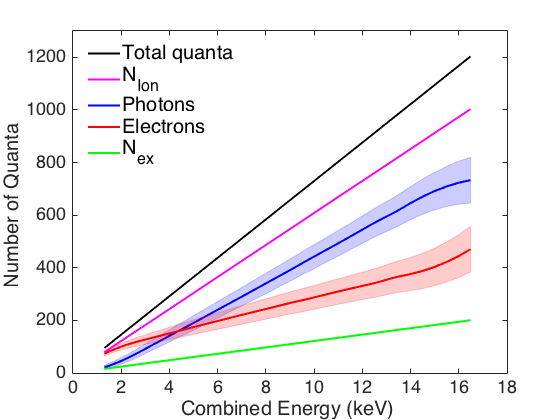
\includegraphics[width=90mm]{fig/quanta-vs-energy.png}
\caption{Top: The mean number of electrons (red) and scintillation photons (blue) produced in LUX at 180~V/cm as a function of energy. The bands indicate the correlated systematic errors on $g_1$ and $g_2$. Also shown are the total number of quanta, primary ions, and primary excitons, assuming an exciton to ion ratio of 0.2. }
\label{fig:quanta-vs-energy}
\end{figure}

\subsection{Recombination at 180~V/cm and 105~V/cm}

We understand the variation of the light and charge yields as being due to recombination, the process by which newly liberated ionization electrons are captured by Xe$^+$ ions, creating additional Xe$^*$ excitons, and ultimately scintillation photons. We model recombination as follows. Starting with a $W$-value of 13.7~eV, we assume that $\alpha$, the initial ratio of excitons-to-ions prior to recombination, is 0.2 independent of energy and electric field~\cite{Doke_alpha}. Then the initial number of ions prior to recombination ($N_{ion}$, equivalent to the initial number of electrons), and the initial number of excitons prior to recombination ($N_{ex}$), and their sum (the total number of quanta), all increase linearly with energy as shown by the solid lines in Fig. \ref{fig:quanta-vs-energy}. Also shown in Fig. \ref{fig:quanta-vs-energy} are the total observed number of electrons and scintillation photons after recombination measured with the LUX tritium data at 180~V/cm as a function of energy. The sum of the observed electrons and photons should also increase linearly with energy, a hypothesis which is tested and confirmed by the tritium spectrum comparison of Fig. \ref{fig:tritium-spectrum}.

As shown in Fig. \ref{fig:quanta-vs-energy}, we find that at very low energy, below 3~keV, the number of electrons and photons is similar to $N_{ion}$ and $N_{ex}$, respectively, while above 4~keV the number of electrons drops below the number of photons, consistent with a large recombination effect at these energies and this electric field. The recombination fraction, calculated according to

\begin{equation}
r = \frac{(n_{\gamma}/n_e) - \alpha}{(n_{\gamma}/n_e) + 1},
\end{equation}

\noindent
is shown explicitly in Fig. \ref{fig:recombination}, measured with both the 180~V/cm and 105~V/cm tritium data. We find only a small difference in the recombination between these two field values in this energy range. It is worth noting that recombination is small at the very lowest energies where the dark matter search is performed, rapidly approaching zero as the energy drops below 4~keV. As noted before, this behavior is of considerable importance for the efficiency of recoil discrimination in LXe~\cite{xed-discrimination}. Other authors have used $\alpha$ values between 0.06 and 0.2~\cite{kaixuan}. Changing the value of $\alpha$ modestly affects the absolute magnitude of the resulting recombination fraction but has only a small affect on the shape as a function of energy. 

\begin{figure}[h!]
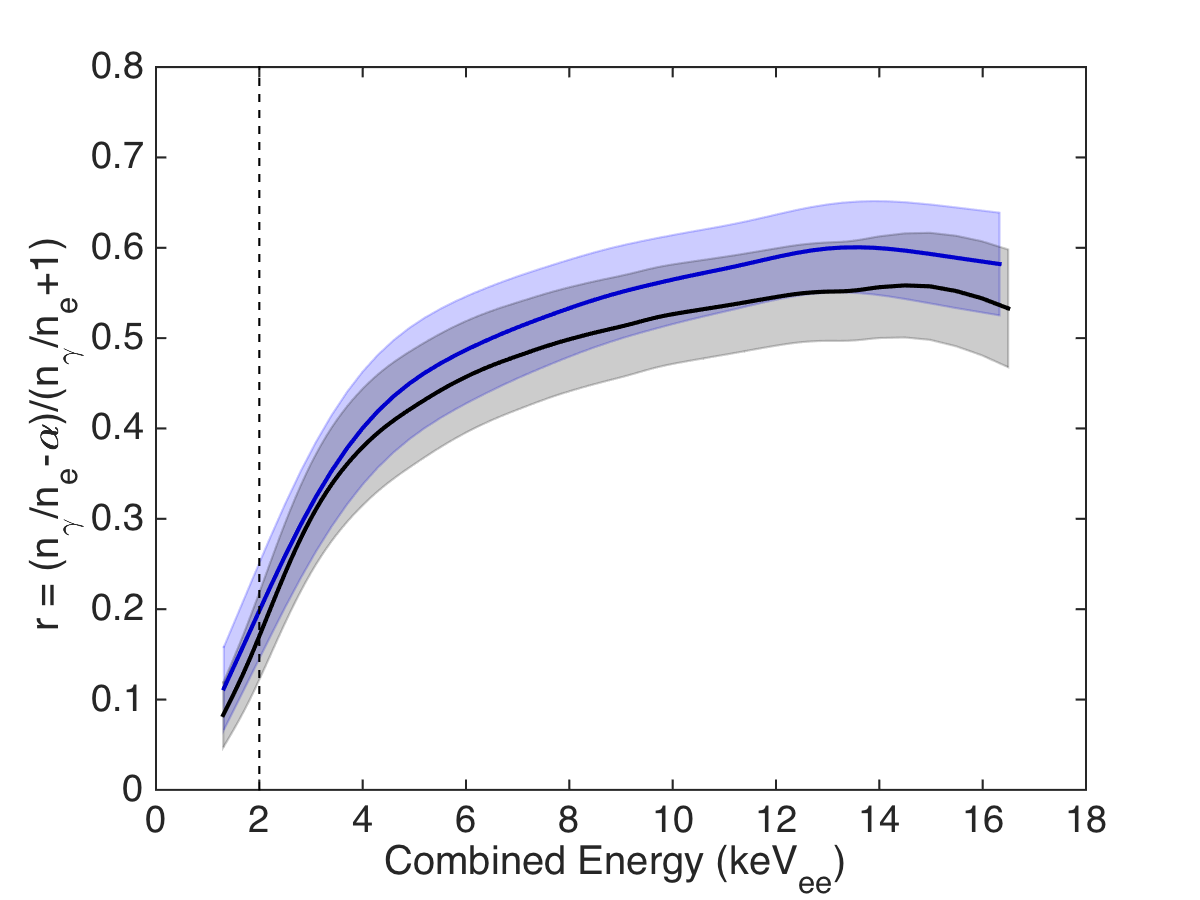
\includegraphics[width=90mm]{fig/recombination.png}
\caption{Recombination fraction of ER events at 180~V/cm (black) and 105~V/cm (blue), assuming an exciton-to-ion ratio of 0.2.}
\label{fig:recombination}
\end{figure}

\subsection{LUX electron recoil band}

The LUX ER band is shown as log$_{10}$(S2/S1) vs S1 in Fig. \ref{fig:ER_band}(top).  It has a characteristic rise at decreasing values of S1 which reflects the rapidly changing charge and light yields below $\sim$6~keV.  Also shown in Fig. \ref{fig:ER_band}(top) is the NR band measured with neutron generator data\cite{DD-paper, lux-reanalysis}. The width of the ER band is of considerable interest because it determines the recoil discrimination of the detector. The leakage fraction ($f$), defined as the fraction of ER events observed below the mean of the NR band, is shown in Fig. \ref{fig:ER_band}(bottom) as a function of S1. The recoil discrimination efficiency ($1-f$) has an average value of 99.81 \% $\pm$ 0.02\% \fixit{ $\rm stat \pm 0.1\%$ sys} for events with S1 between 1 and 50 phd.

\begin{figure}[h!]
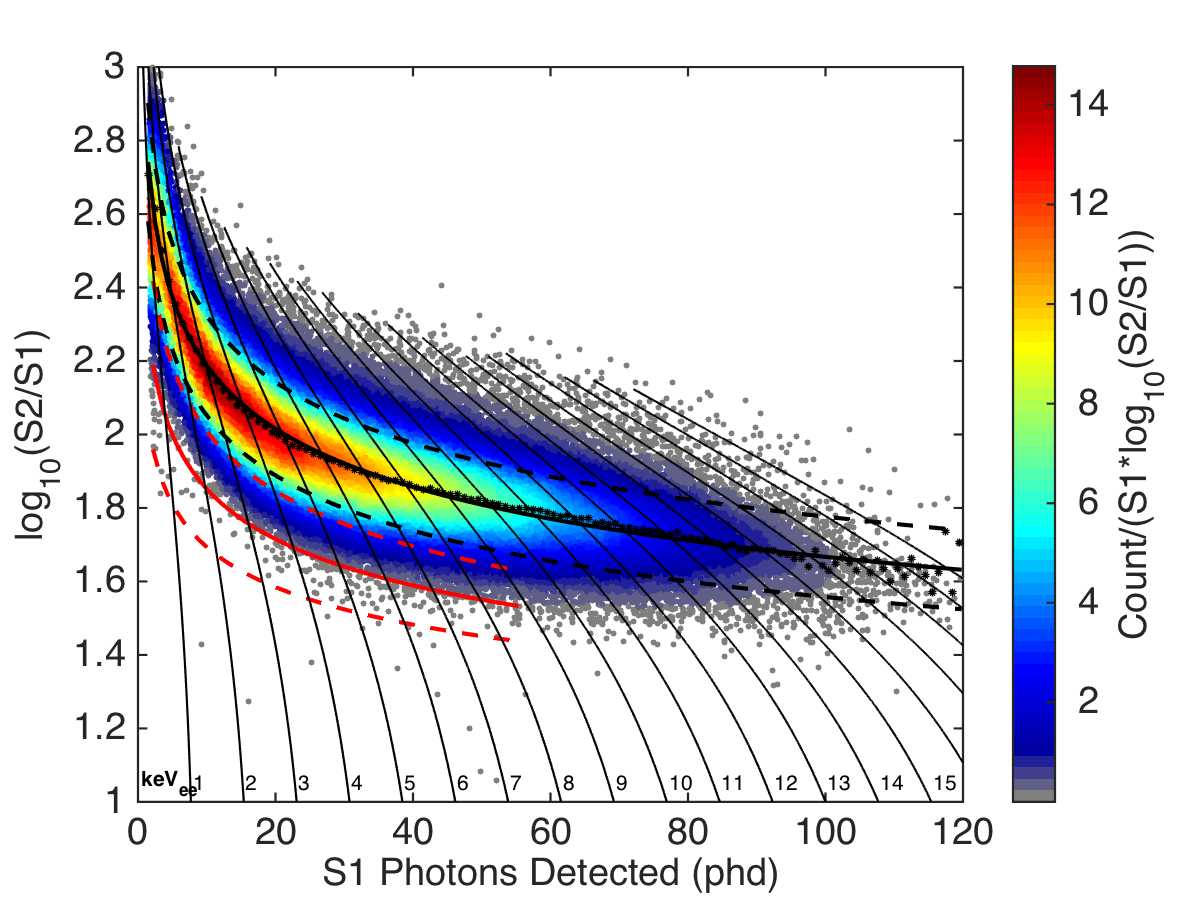
\includegraphics[width=80mm]{fig/CH3T_ER_Band.png}
%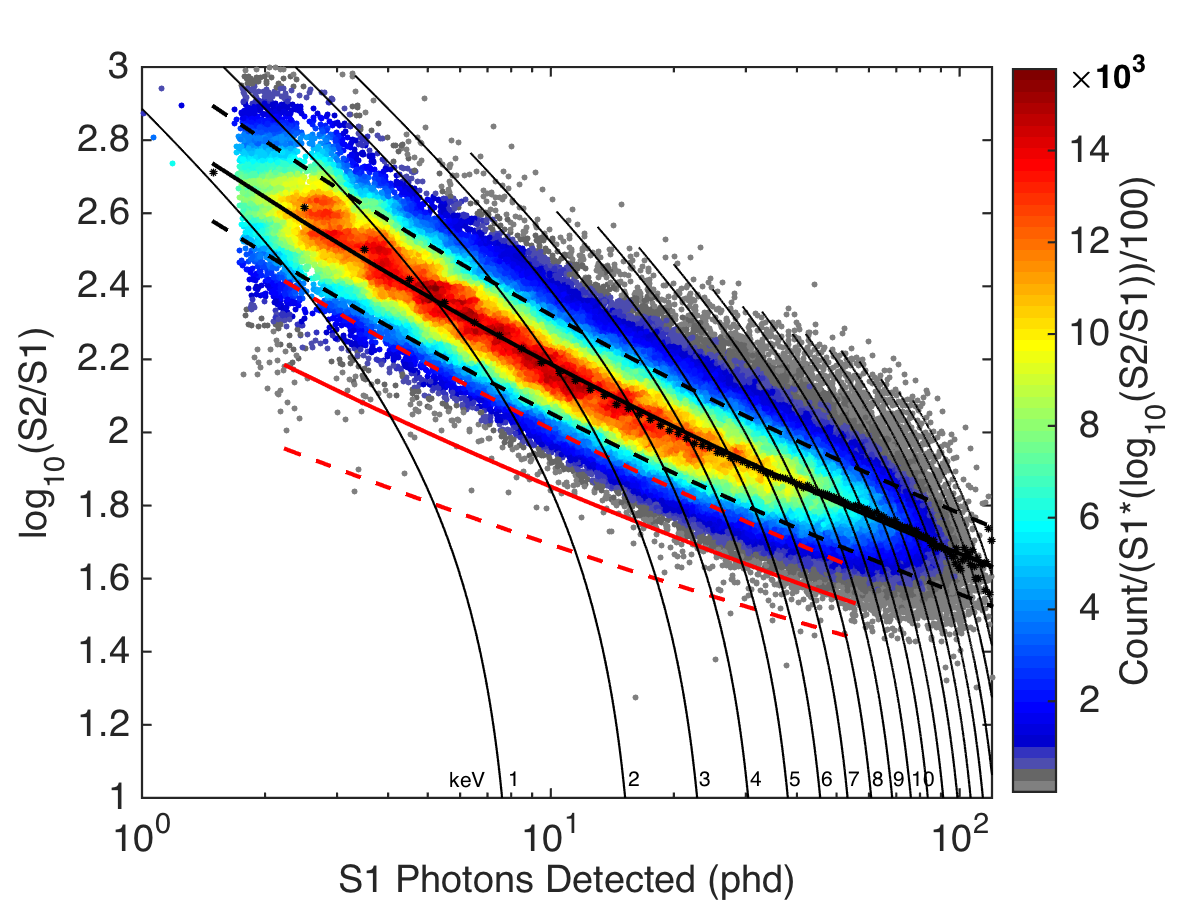
\includegraphics[width=80mm]{fig/CH3T_ER_Band_log.png} .... log version
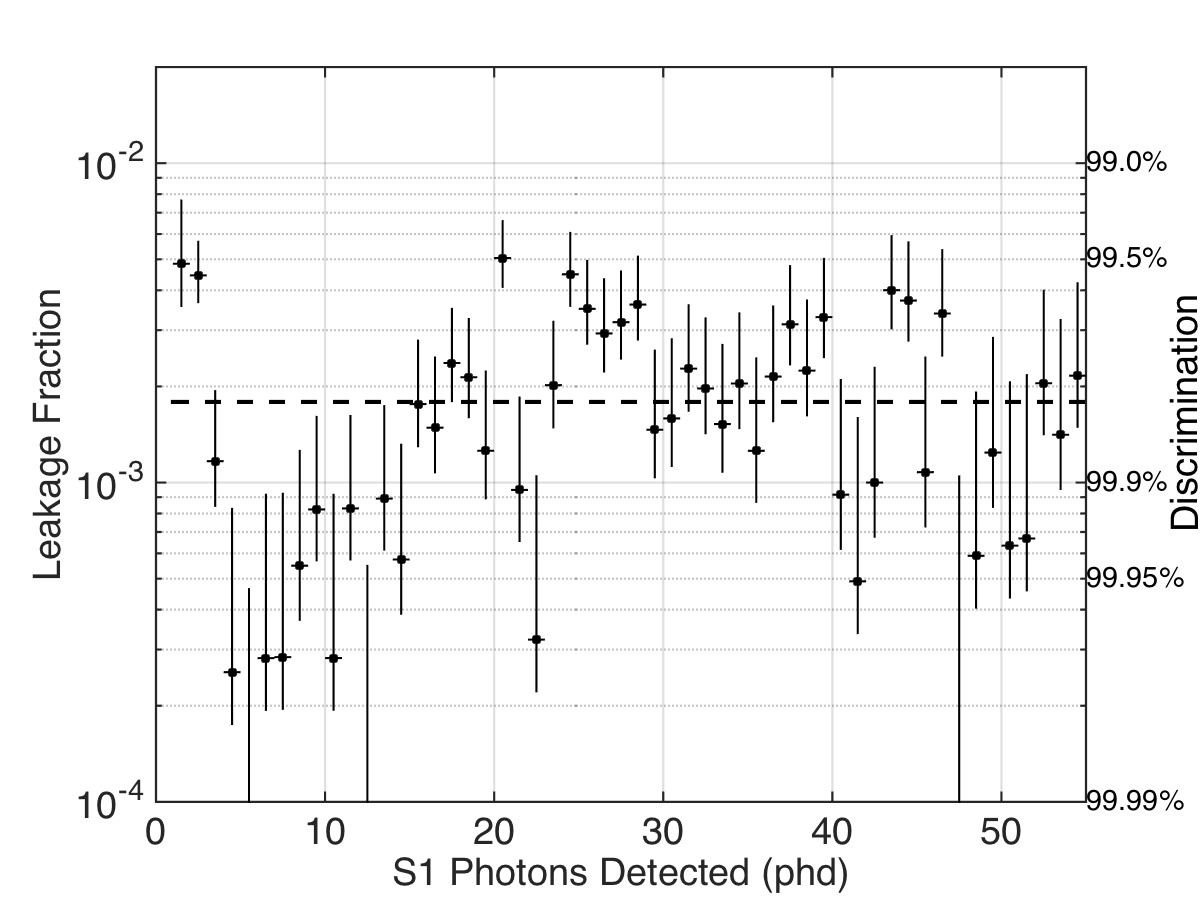
\includegraphics[width=75mm]{fig/CH3T_Leakage_Run03.png}
\caption{Top: The electron recoil band of LUX illuminated by 170,000 tritium events at the nominal LUX electric field of 180~V/cm.  The recoil discriminant variable, log(S2/S1), is shown vs. S1 between 1 and 120 phd in S1 (with contours of constant energy from 1 to 20~keV). Also indicated in black are the mean and the 10\% and 90\% contours of the ER population. The solid red line represents the mean NR band determined with DD neutron generator data. The dashed red indicates the 10\% and 90\% contours of the NR band. Bottom: Observed LUX recoil discrimination vs. S1, defined as the fraction of events below the NR mean. Y-axis labels: left -  leakage fraction ($f$); right - discrimination ($1-f$).}
\label{fig:ER_band}
\end{figure}

In general the ER band width should be comprised of three components: the uncertainties on  $n_{\gamma}$ and $n_e$  due to detector resolution ($ \sigma(n_{\gamma})$ and $ \sigma(n_e)$), and true event-to-event variations in recombination ($ \sigma(R)$). $ \sigma(n_{\gamma})$ and $ \sigma(n_e)$ are responsible for fluctuations in the vertical  and horizontal directions in Fig. \ref{fig:tritium-scatter},  while $ \sigma(R)$ causes fluctuations along the diagonal lines of constant energy. $ \sigma(n_{\gamma})$ and $ \sigma(n_e)$ can be measured as a function of energy and are shown in Fig. \ref{fig:recomb-flucs} for LUX tritium data at 180~V/cm\cite{Dobi_Thesis}. Also shown in Fig. \ref{fig:recomb-flucs} is the extracted value of $ \sigma(R)$ as a function of energy after controlling for $ \sigma(n_{\gamma})$ and $ \sigma(n_e)$ by a method described in Ref. \cite{Dobi_Thesis}. \fixit{The amount of event-to-event recombination fluctuations ($ \sigma(R)$) grows linearly as a function of number of ions available for recombination (or energy). For energies between 2 to 16~keV the size of recombination fluctuations can be described by $\rm \sigma(R)=(0.07\pm0.01) \times n_{ion}$, consistent with \cite{Dobi_Thesis}.}

\begin{figure}[h!]
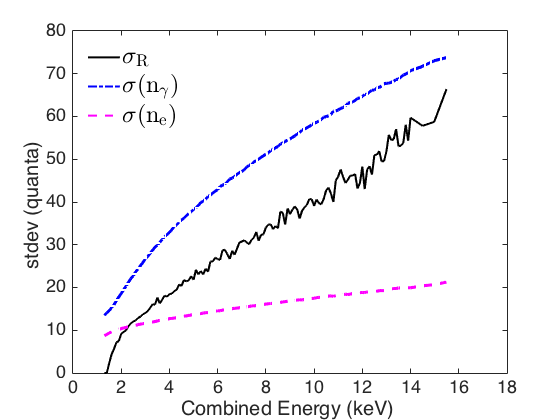
\includegraphics[width=90mm]{fig/recomb_flucs.png}
\caption{Black: recombination fluctuations in LXe measured with LUX tritium data at 180~V/cm. Dot-dash blue: Detector resolution for counting photons. Dashed magenta: Detector resolution for counting electrons.}
\label{fig:recomb-flucs}
\end{figure}

We find that at 180~V/cm in LUX, $ \sigma(n_{\gamma})$ is the most important contributor to the ER band width over the entire tritium energy spectrum. Between 2 and 6~keV, where the WIMP search is most sensitive, $ \sigma(n_e)$ and $ \sigma(R)$ are of comparable magnitude and secondary importance. We note that an ideal detector would be limited by only $ \sigma(R)$.

The statistical description of the width of the LUX ER band is relevant to the WIMP search profile likelihood fit. To study the band width in more detail, in Fig. \ref{fig:ER-Gauss} we histogram log$_{10}(S2/S1)$ in 16 bins of S1 from 1 to 49 phd and with a bin-width of 3 phd. In each bin, we show a Gaussian fit to the data after subtracting the centroid and dividing by the Gaussian width. We find that the Gaussian fits describe the data well out to $2\sigma$ on the upper side and $3\sigma$ on the lower side, beyond which non-Gaussian tails are visible.  We have investigated the origin of these tails. On the lower side, which is most directly relevant to the WIMP search, the largest non-Gaussian tail is found in the lowest S1 bin (1 - 3 phd). This tail is reproduced in simulation and originates from Poissionian fluctuations in the counting statistics. The origin of the non-Gaussian tails on the upper side is less clear, but fluctuations in the charge extraction efficiency at the liquid-gas interface are a possible explanation.

Several outlier events are also evident in Fig. \ref{fig:ER-Gauss}, particularly at low values of log$_{10}(S2/S1)$. Although these events are rare in this dataset, their origin is of considerable interest for understanding the WIMP sensitivity of future LXe experiments.  Therefore we have investigated whether these events are attributable to detector pathologies, to backgrounds, or to the fundamental recombination physics of the LXe . In this dataset we expect to find about 0.5 low (S2/S1) events due to ion recoil from $^{210}$Pb decay on the interior TPC walls. These events can have an improperly reconstructed radial position that allows them to pass our fiducial cuts.  Another possible background are accidental coincidences between two distinct tritium events. In this scenario, an S1 from a tritium event below the cathode, and thus not having an S2, is improperly paired with a low energy tritium S2 in the fiducial volume for which the S1 signal fell below threshold. The expected number of such events in the tritium dataset is 2.5. The tritium dataset used here contain 27.5 live hours of data, during which time we expect to have 15 non-tritium events from the LUX ER background rate between 1 and 18 keV. These events should occur near the mean of the tritium ER band and should not be observable in this dataset. The total background expectation for low (S2/S1) events is therefore three, and in Fig. \ref{fig:ER-Gauss} we find roughly three highly isolated low (S2/S1) events. We conclude that the number of low (S2/S1) outlier events is consistent with the background expectation.

\onecolumngrid
\break
\begin{figure}
%\begin{sidewaysfigure}[p!]
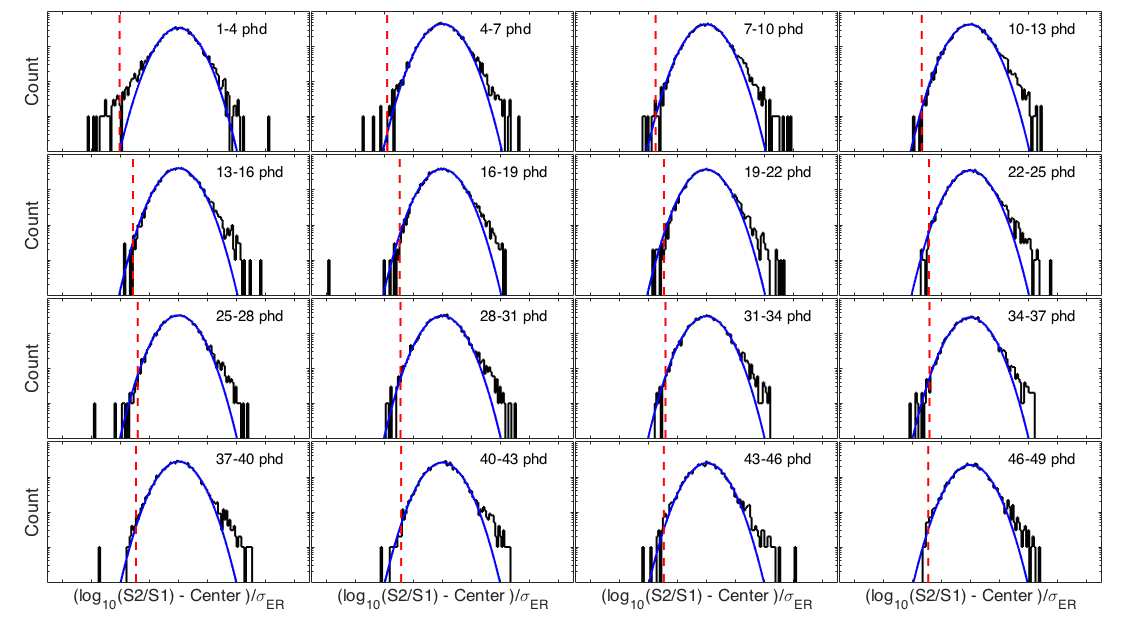
\includegraphics[width=140mm]{fig/Gaussianity/GaussER_all.png}
\caption{Electron recoil population from tritium events in 3 phd bins over over the WIMP region of interest (1 - 49 phd). We fit each bin to a Gaussian, and subtract the centroid of the Gaussian. The x-axis is measured in units of the fitted Gaussian width. The red dashed line represents the mean of the NR band in each bin. }
\label{fig:ER-Gauss}
%\end{sidewaysfigure}
\end{figure}
%\break
\twocolumngrid

